% id: 124-23
% book: 100발100중 3-2 기말 · 01 3-2 기말(원의 성질·통계·부록)
% section: 고난도 기출문제
% figure: crop:fig-124-23.png
% answer: ①
% answer_source: 답지(빠른정답)
% variant_level: 0 (원본 전사)
% 이 파일은 build.mjs 가 items.json 에서 만든다. 고칠 때는 items.json 을 고친다.
\smash{\raisebox{1.5mm}{\dmkichul{100발100중 3-2 기말 124쪽 23번}}}
\noindent\begin{minipage}[t]{0.58\linewidth}\vspace{0pt}\raggedright 그림은 민재네 반 학생 $25$명의 두 차례에 걸친 $50\mkern3mu \mathrm{m}$ 달리기 기록을 조사하여 나타낸 산점도이다. $1$차와 $2$차 기록의 평균으로 순위를 정할 때, 상위 $20\mkern3mu \%$ 이내에 드는 학생들의 $2$차 기록의 평균은?\end{minipage}\hfill\begin{minipage}[t]{0.4\linewidth}\vspace{0pt}\centering 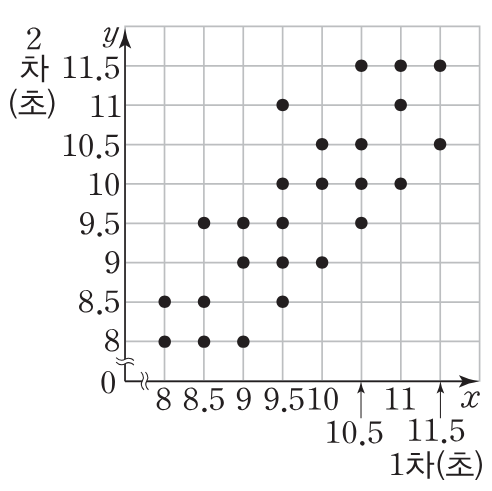
\includegraphics[width=117.9pt]{figures/fig-124-23.png}\end{minipage}\par
\begin{choices32}{$8.2$초}{$8.25$초}{$8.4$초}{$11.1$초}{$11.2$초}\end{choices32}
